\chapter{Introduction}
\label{introduction}

% What is the problem: necessity of supplying consistent sources in nuclear and hospitals etc 
In a safety-critical application, the failure or malfunctioning of equipment can result in loss of life, serious injury or damage to the environment\cite{HayekSafety, Borcsok}. For example, the failure of hospital equipment can be fatal. In these environments, the effects of power cuts can be devastating\cite{azeem, onipede}. The reliability of the supply of power to these systems is essential especially with recent trends towards renewable sources for which a consistent supply to applications cannot be guaranteed\cite{liserre, onipede}.

% what is the solution to this problem
An Automatic Transfer Switch (ATS) is a device that ensures a reliable power source is available to critical loads in a system\cite{azeem}. This involves monitoring two separate sources and switching between them if necessary. ATS devices have been adopted in a number of environments, including nuclear and medical, to ensure that safety-critical operations can be performed. Consequently, in the development of ATS systems, functional safety and verification are imperative to guarantee that the critical loads are transferred appropriately.

This report describes the design, implementation and verification of a new ATS processor for use in safety-critical applications. All work described in this report was carried out as part of the MEng project for the Socomec Group. Socomec was established in 1922 in Alsace, France, specialising in the control and security of electrical supplies. Currently, there are 28 subsidiaries around the world and have a turnover of 537 million euros. This project was conducted in the global headquarters in Benfeld, France.

%Additional measures must be taken and safety-related standards must be followed to ensure that the system operates correctly. 

\section{The Socomec ATyS}
% what is the current design
The Socomec Group product range includes a microcontroller-based ATS device. An example ATyS, the commercial name given to Socomec ATS devices, can be seen in Figure \ref{AtysDevice}. The Socomec range can handle a range of power supplies from 125A to 3200A\cite{socomec_atys_range}. It is implemented using two control boards: the first is used to monitor the supplies and determine whether it is necessary to perform a transfer, the other board is responsible for performing the physical switch between the supplies by driving a universal motor. Each of these control boards use a microcontroller as the processor.
% atys connection / configuration
An example network configuration of the ATyS, where it controls the connection of the circuit between a mains power supply and a back-up generator, is shown in Figure \ref{AtysConfig}. Several configurations are possible for the ATyS but the principle remains the same: ensure a reliable supply of power.

\begin{figure}[h]
\centering
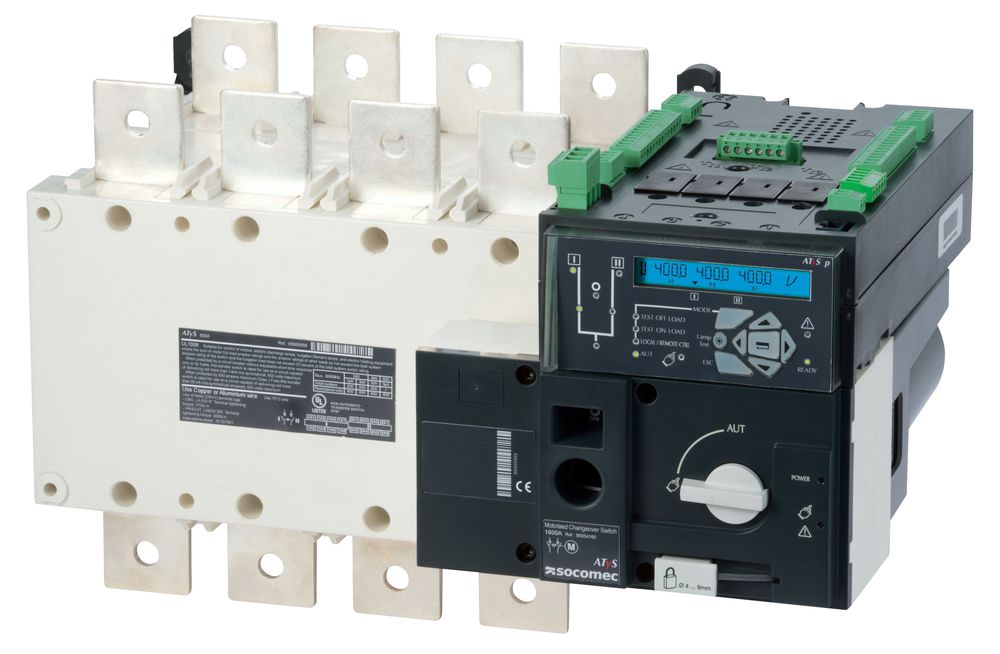
\includegraphics[width=0.6\textwidth]{images/ATySDevice.jpg}
\caption{The Socomec Automatic Transfer Switch (ATyS)\cite{socomec_atys}}
\label{AtysDevice}
\end{figure}


\begin{figure}[h]
\centering
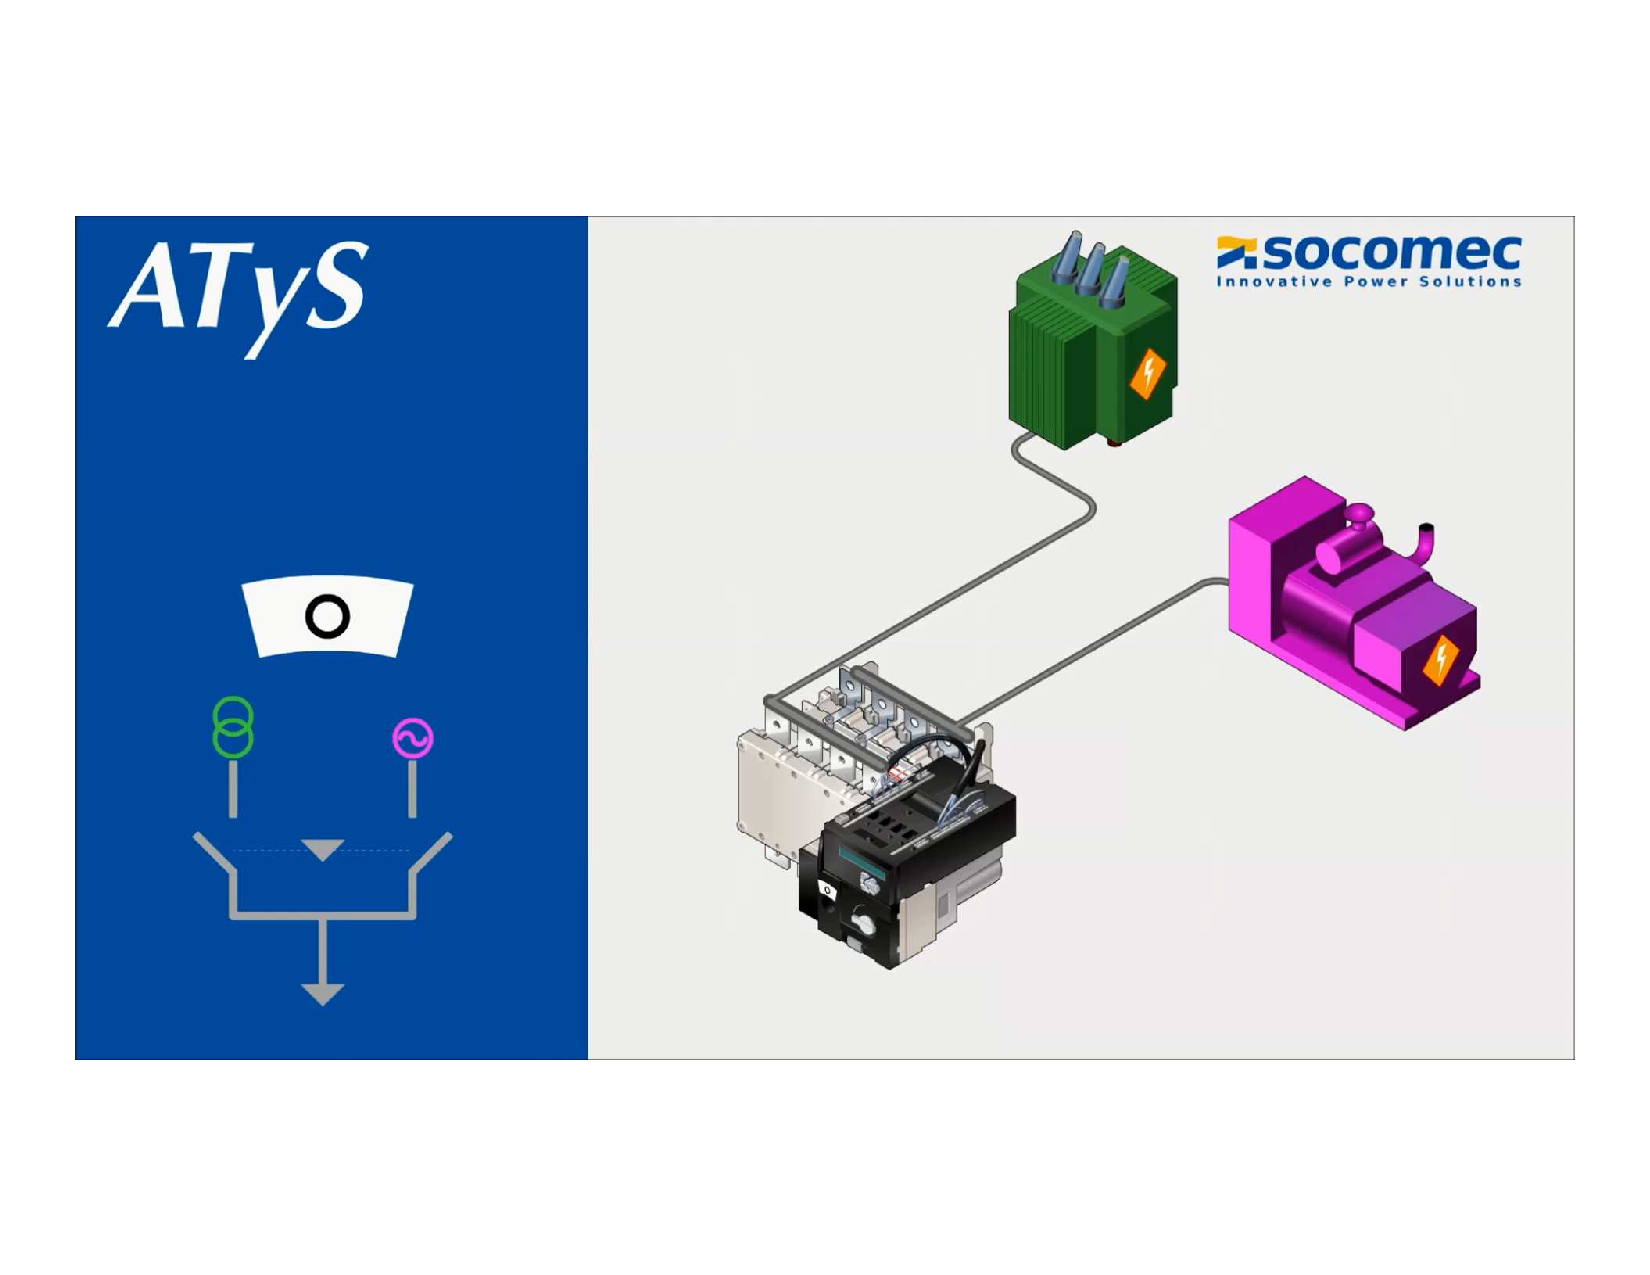
\includegraphics[width=0.7\textwidth]{images/AtysConfig.pdf}
\caption{Example ATyS configuration controlling a load connection between mains (green) and a back-up generator (pink)\cite{socomec_atys_network}}
\label{AtysConfig}
\end{figure}


\section{Project Aims}

% what change is being made to the design and why
The project, outlined in this report, involves replacing the micro-controller processor in the ATyS motor control board with a Field Programmable Gate Array (FPGA). The primary motivation for this change is to enhance the functional safety of the ATyS system where functional safety is defined as "ensuring the correct behaviour of a system and detecting or correcting when the behaviour is not as expected"\cite{Jeppesen, IECfunctionalsafety}. 
% nature of the project (proof of concept, investigation into safety requirements (e.g. verification), prototype (design) with focus on the safety function of the device)
The overall aim of the project is to investigate the advantages of an FPGA-based solution with a focus on the functional safety of the device. In order to do this, the project had the following objectives:
\begin{itemize}
  \item Conduct a literature review to discover where FPGAs have been used in similar systems
  \item Analyse the related safety standards and determine how they could be applied to an FPGA-based system
  \item Design an FPGA-based alternative solution from the existing micro-controller specification
  \item Develop VHDL code to implement the design using processes and tools recommended by the safety standards  
  \item Verify the design in accordance with the recommendations of the safety standards
  \item Physically prototype the FPGA-based solution and compare the response with the original solution
\end{itemize}

%This will involve the development of a PCB with an FPGA processor onto which a VHDL design will be synthesised.   

% comparison with the existing solution: how will the project be evaluated

\section{Report Structure}
% how the report will be structured
This report will begin by reviewing literature in areas relevant to this project. As part of this, the theory behind the chosen methodologies for this project is presented and similar projects are discussed. Following this, the design and implementation of the prototype FPGA-based system are presented in Section \ref{design}. The verification of this design is then presented in Section \ref{verification}. The behavioural results of the prototype are discussed and compared against the existing solution in Section \ref{results}. The results of the project are evaluated in Section \ref{evaluation} against the initial aims and objectives outlined in this section and suggestions for further work are presented. Finally, the conclusions drawn from the project are summarised.
